\documentclass[12pt]{article} \usepackage[margin=1in]{geometry}

\usepackage{graphicx}
\usepackage{color}

%% \usepackage{amsmath}
%% \usepackage{listings}

%% \lstloadlanguages{C++} \lstset{ language=C++, breaklines=true,
%%   keywordstyle=\color{blue}, commentstyle=\color{red} }


\newenvironment{listing}%
               {\begin{table}
                   \begin{tabular}{ p{6in} }
                     \hline}%
               {\end{tabular}%
               \end{table}}


\begin{document}

\title{A New Algorithm for Second Order Perturbation Theory}
\author{Andrey Asadchev \and Mark S. Gordon}
\date{}

\maketitle


\abstract{
A new second order perturbation theory (MP2) algorithm is presented
for closed shell energy evaluations. The new algorithm has a
significantly lower memory footprint, a lower FLOP (floating point
operations) count, and a transparent approach for the disk/distributed
memory storage of the MP2 amplitudes. The algorithm works equally well
on single workstations and large clusters. The new algorithm allows
one to perform large calculations with thousands of basis functions in
a matter of hours on a single workstation. While for most practical
purposes, classical MP2 is eclipsed by density-fitting methods, the
approaches and lessons learned in the presented implementation are
applicable beyond the MP2 algorithm.
}


\section{Introduction}
The integral transformation, also known as 4-index tranformation,
tranforms atomic (typically) integrals to molecular integrals via the
simple formula:

$$(ij|kl) = C(i,p)C(j,q)C(k,r)C(l,s)(pq|rs)$$

Using the common convention, occupied indices $o$ are designated by
indices $i,j,...$, virtual indices $v$ are designated by indices $a,
b,...$, and atomic indices $n$ by indices $p,q,r,s$.

Typically, several classes of molecular integrals are needed, eg
$(ai|bj)$, $(ab|ci)$, etc.  But in the case of MP2 energy,

$$t_{ij}^{ab} = \frac{2 (ai|bj) - (bi|aj)}{\epsilon_i + \epsilon_j - \epsilon_a -
  \epsilon_b}$$
$$E_{MP2} = \sum \sum t_{ij}^{ab}(ai|bj)$$

only $(ai|bj)$ integrals are needed to form $t_{ij}^{ab}$ MP2
amplitudes.  The $(ai|bj)$ integrals and consequently $t$ amplitude
have symmetry such that $(ai|bj) = (bj|ai)$ which can be used to halve
storage requirement and number of computations.

The MP2 energy calculation scales as $O N^4$ and requires $O^2 V^2$
integral storage. Out of all many body methods is the cheapest and the
one with lowest compute to I/O ratio.

There is a number of different algorithms developed over the years,
\cite{head1988MP2, frisch1990semi, wong1996parallel,schutz1997integral,
  fletcher1997parallel, ford2007array, ishimura2006new}
due to simplicity of the algorithm and its popularity.
This work is to improve the algorithm and generalize it to handle
larger calculations, using either memory or filesystem as a storage
medium.

\section {Matrix chaining}
There exists a simple matrix chaining multiplication property, which,
surprisingly, is not very well-known.  Given three (or more) matrices,
the matrices can be multiplied without changing the outcome by two
different factorizations, $A = (BC)D$ and $A = B(CD)$.

At first glance the above fact is not interesting until you consider
the number of operations between the two.  Suppose for example, that
the dimensions are $B(k,l)$, $C(l,m)$, $D(m,n)$, and $A(k,n)$.  The
number of operations are $(klm + kmn)$ and $lmn + kln$ respectively.

This property can be applied to drastically reduce the number of
operations in integral transformations.  Suppose the integral
transformation is applied in the naive order:

$$G(v,o,v,o) = C(o,n)(C(v,n)(C(o,n)(C(v,n)G(n,n,n,n))))$$

then the total number of operations is:

$$v n^4 + v o n^3 + v^2 o n^2 + v^2 o^2 n = v n (n^3 + o n^2 + v o n +
vo^2)$$

if the transformations are applied occupied index first, then the
number of operations is:

$$o n^4 + o^2 n^3 + v o^2 n^2 + v^2 o^2 n = o n (n^3 + o n^2 + v o n +
v^2 o)$$

and the difference between the two is on the order of a factor of
$v/o$.  Considering that typically $v > o$, the computational savings
are significant.

To second benefit comes from reduced memory requirements.  Since the
first two transformations ``shrink'' atomic indices to occupied
indices, the entire tensor is quickly reduced to $G(o,o,n,n)$ storage,
rather than much larger $G(v,o,n,n)$ storage.

\section{General Algorithm Considerations}
To have a scalable algorithm, a special attention needs to be paid to
memory footprint, I/O patterns, and I/O optimization by means of
aggregation of smaller transfers into larger blocks.

\subsection {Memory}
The algorithm must have small memory print, under 1G per core on
current hardware, even for large computations with several thousand
basis functions.  In terms of basis functions and shells, the memory
overhead must be on order of $M^2O^2$, where M is some adjustable
blocking factor, for example the size of largest shell in the basis
set, otherwise any significant computation would require nodes with
ten or more gigabytes of memory per {\it core}.  For example, a
computation with 3000 basis function and 300 occupied orbitals
requires 22GB per {\it core} if memory were to scale as $N^2O$.  The
blocking factor must be adjustable to adapt to computers with
different number of cores and memory.

\subsection {I/O Considerations}
For any significant problems size, the amplitudes are too great to
store in core memory.  GAMESS \cite{gamess}, for example has several MP2 algorithms,
including two which are parallel disk-only \cite{ishimura2006new}
and distributed memory \cite{fletcher1997parallel}
implementations.  However, using modern programming techniques, the
same algorithm can be adapted to both, disk and distributed memory.
The efficient access patterns between distributed memory and disk are
the same: large contiguous transfers are preferred.  Typically disk
has much worse throughput than the distributed memory.  If an
algorithm works well with disk, it is guaranteed to work well with
distributed memory, even when running over slow Ethernet networks.

The general efficacy for using disk is outlined by Pulay \cite{ford2007array}.
  In short,
smaller research groups may not have access to computers with large
memory, but access to workstations with large fast disks is very common.

There is one important detail: due to buffering, writes tend to be
significantly faster than reads.  Therefore, algorithms which both
read and write large datasets should be optimized in favor of reads.

The latency of storage access can be hidden by overlapping I/O and
computations.  This can be accomplished either by having a number of
threads perform computations and I/O independently of one another or
having a single I/O thread perform data transfers while the other
thread perform computations.

Implementation transparency, e.g. distributed memory or file
implementation, is easily accomplished using polymorphic interface,
e.g. overriding virtual functions in C++, allowing to choose an
appropriate implementation at the runtime.  For example, use 
distributed memory if enough is available, otherwise default to
filesystem backend.

\subsection{File I/O considerations}
There are two de facto file format and their corresponding libraries
that allow easy manipulation of multidimensional scientific data on
filesystem, HDF5 \cite{hdf5} and NetCDF\cite{netcdf}.
For the purposes of implementing dense
tensor storage, the two file format are comparable in performance and
capabilities.

Storing data on the single node is straightforward.
However parallel storage requires parallel file system.  There are
number of parallel filesystems, for example PVFS and Lustre.  PVFS is
easily configurable filesystem, suitable for local clusters.  Lustre
is more complicated filesystem, found for example on Cray
supercomputers.  Regardless of particular filesystem, the principle is
similar to that of RAID0 \cite{patterson1988case}: an entire file is stripped over a number of I/O
nodes.  The performance of parallel filesystem primarily depends on
the strip size and the number of I/O nodes.  Both  HDF5 and NetCDF
have facilities  for parallel I/O.

\section{Naive Approach}

A simple MP2 approach is described in listing \ref{naive}.

%\begin{lstlisting}[label=naive, caption=Naive approach, numbers=left]
\begin {listing}
\begin {verbatim}
allocate V(O*O/2,N,N); // (ia|jb) storage
for S in Shells {
  for Q <= S {
    for R in Shells {
      for P in Shells {
        // skip insignificant ints
        if (!screen(P,Q,R,S)) continue;
        t1(i,R,Q,S) = eri(P,Q,R,S)*C(i,P);
      }
      t2(i,j,Q,S) = t1(i,R,Q,S)*C(j,R);
    }
    // exploit symmetry
    V.store(t2(ij,Q,S));
    V.store(t2(ji,S,Q));
  }
}
// 3rd index
for s in N {
  t2(ij,Q) = V(ij,Q,s); // load NO^2 tile
  t3(ij,a) = t2(ij,Q)*C(a,Q); // transform
  V(ij,a,s) = t3(ij,a)); // store VO^2 tile
}
// 4th index + energy computation
for a in V {
  t3(ij,S) = V.load(ij,a,S); // load NO^2 tile
  t4(ij,b) = t3(ij,S)*C(b,S); // transform
  E += Energy(t4); // evaluate energy
}
\end{verbatim} \\
\hline
\caption{Naive approach}
\label{naive}
\end{listing}

The main points about the simple implementation:
\begin{itemize}
\item The amplitude symmetry is exploited in Q,S shells.  The half
  transformed integrals $t2$ are writen as triangular matrices, $i <=
  j$ as well as its transpose $j <= i$.  If running on multiple cores,
  each Q,S pair can be evaluated independently, allowing to benefit
  from overlapping computation/write.
\item Integral computation and first transformation are screened
  using Schwarz method.  Subsequent transformations are not screened.
\item The matrix transformations can be done using BLAS matrix
  routine.  Several shells can be transformed at the time to increase
  efficiency.  The temporary memory is on the order of $(O^2 M^2)$.
\item 3rd tranformation is straightforward, temporary memory required
  is $(O^2*N/2)$ where $N$ is the number of functions.
\item the fourth transformation requires noncontiguous read.  As
  mentioned above, the disk is not efficient to handle noncontiguous
  read.  For a large problem, the 4th step becomes increasingly slow,
  rendering this approach extremely inefficient.
\end{itemize}

\section{Better Algorithm}
What is desired is an algorithm which still exploits symmetry but is
somehow able to load untransformed index contiguously to maximize
throughput.

If the amplitudes were stored as $t(N*N,ij)$ arrays then it would be a simple
matter of reading contiguous blocks corresponding to an occupied
index, transforming them, and evaluating energy, all at a cost of
single read only.  Keep in mind that the quantity $N*N$ is a
relatively small, only 200MB for 5000 basis functions.

The problem is then how to write such data efficiently since it is
generated as $(ij,Q,S)$ shell pair at the time.  Writing individual shell pairs
at a time to form $(QS,ij)$ is inefficient, for example in the case of
s-shell pair, it would require a long noncontiguous write.  However
one can notice that to generate occupied transformation, very little
memory is needed.  This fact can be exploited to evaluate and to write
a block of $M^2$ functions at a time.  For example, assuming 500 occupied
orbitals, working memory required is 1MB per shell function, therefore
a block $M^2$ of 256 functions, e.g. 16 sp-shell pairs, is only 256MB but 16
separate writes can now be aggregated into a single large write.

By performing $(QS,ij)$ and its symmetric transpose $(SQ,ji)$ next to
each other, the contigous section of write can be further doubled.

The fact that the virtual index transformation is also relatively
small in terms of memory can be used to further improve I/O.  If an
entire {\it node} has 2 GB of memory, 10 $(Q,S,ij)$ blocks can be
loaded at once.  This means the tensor storage can be redimensioned
from $(N*N,O^2/2)$ to $(B*N*N,O^2/(2B))$, with $B=10$ in the example,
and consequently the writes can now be $(B*QS,ij/B)$, with atomic and
occupied orbitals interleaved.  If $B = O^2/2$ then the algorithm is
essentially in-core version. 
The graphical depiction of the access patterns is outlined in figure
\ref{patterns}.

\begin{figure}[here]
\begin{center}
%% 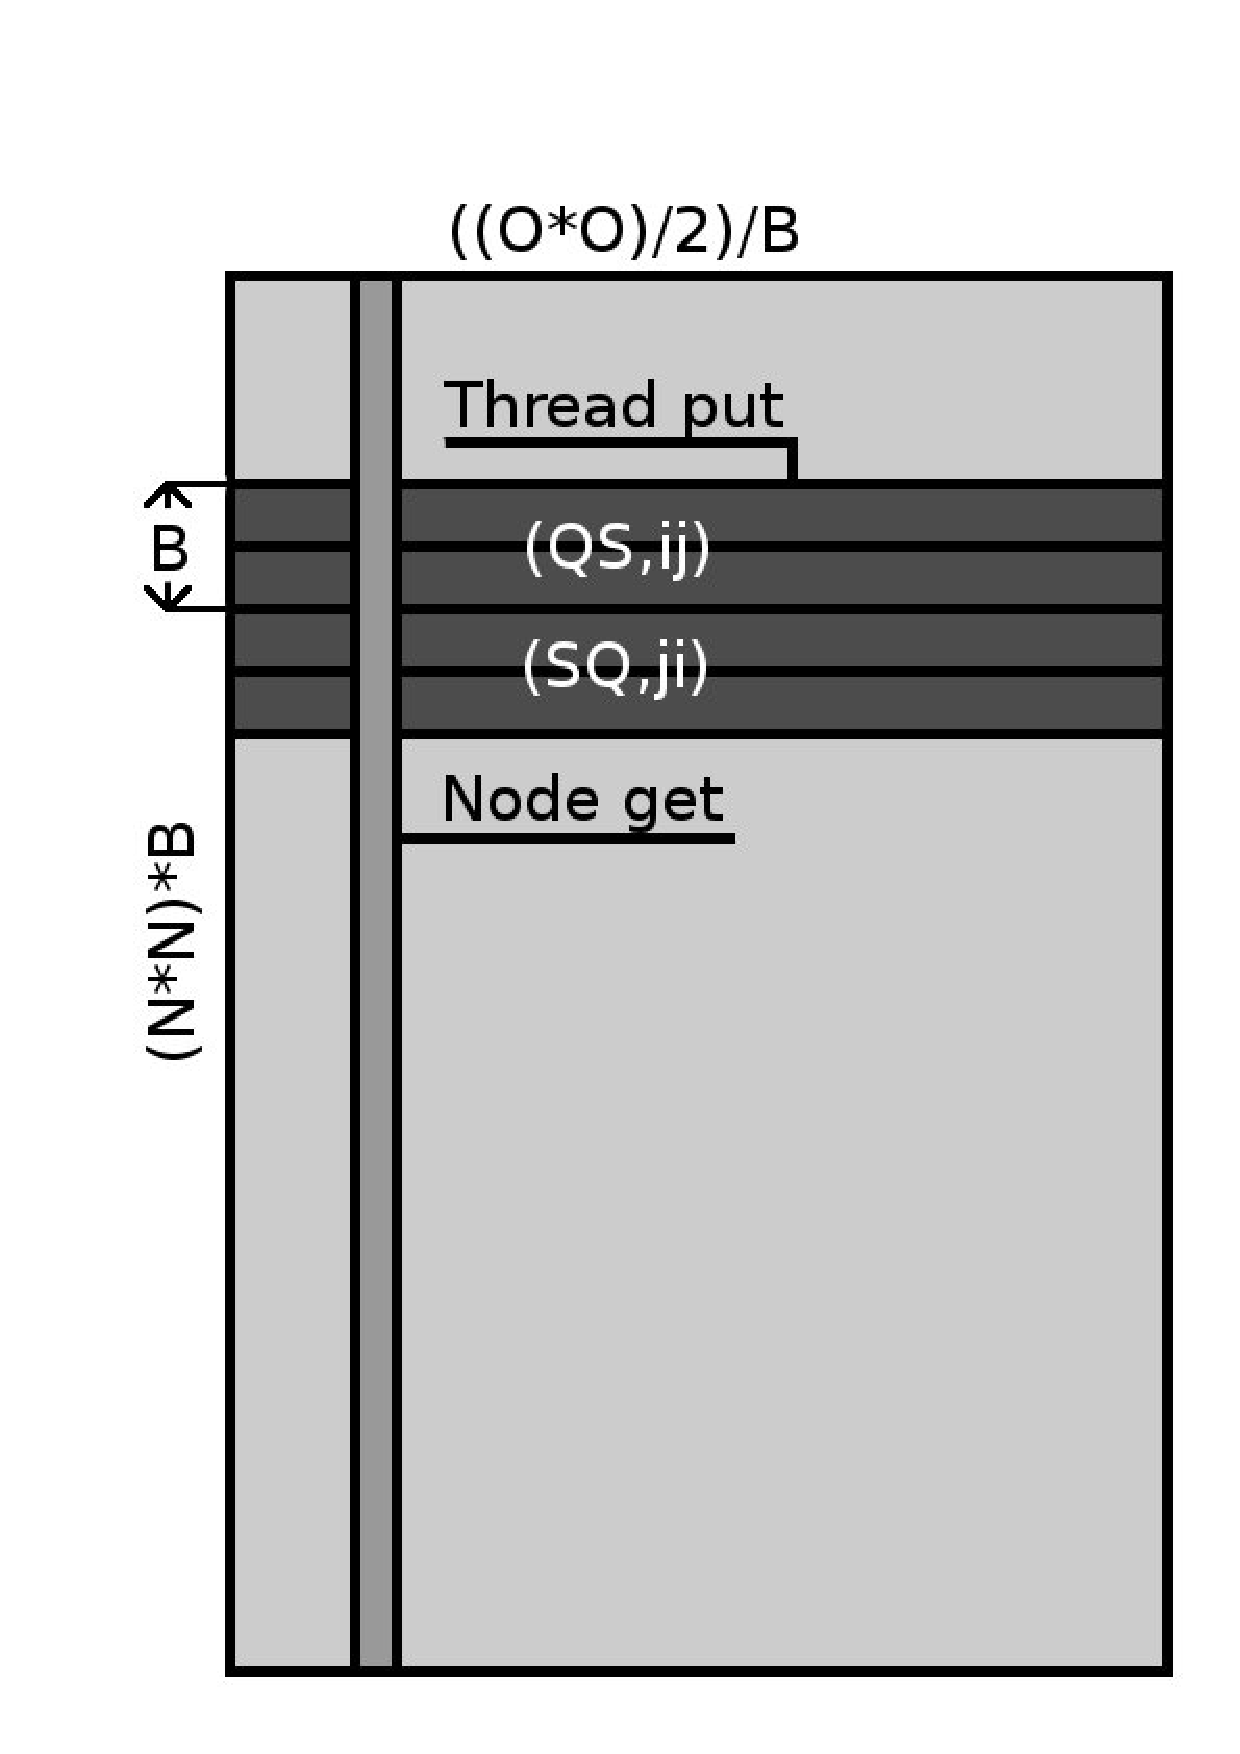
\includegraphics[scale=0.25]{figure.pdf}
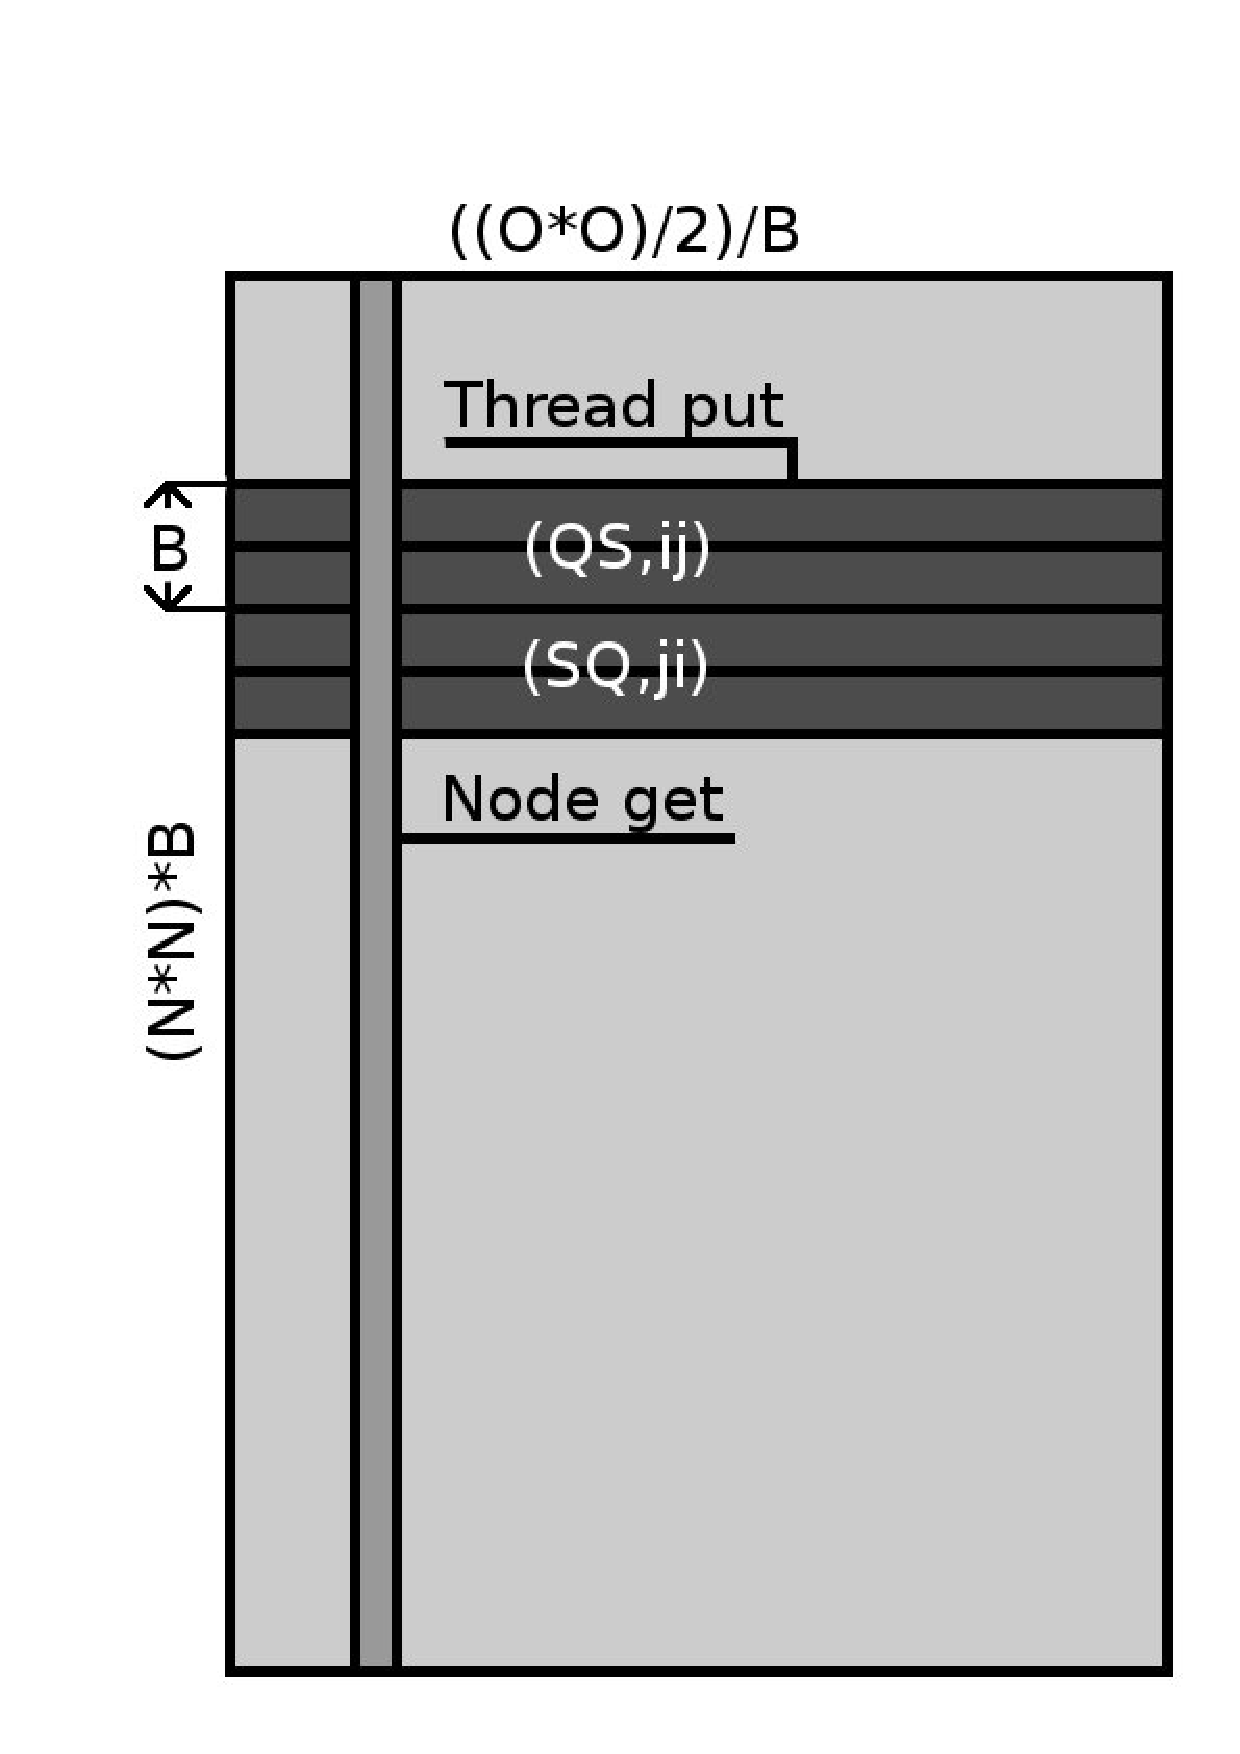
\includegraphics[scale=0.25]{figure.pdf}
\caption{Amplitude access patterns}
\label{patterns}
\end{center}
\end{figure}

Combining the above ideas, one can develop the following
algorithm, which has $(2*M^2*B,ij/B)$ and $(N^2B)$ I/O respectively,
Listing \ref{better}, with $M$ and $B$ factors determined by setting
runtime memory limits.

%\begin{lstlisting}[label=better, caption=Better approach, numbers=left]


\begin{listing}
\begin{verbatim}
B = ...; // some blocking factor, according to available memory
allocate V( N*N*B, (O^2/2)/B );
for (S,Q) in Blocks(Q <= S, M) {
  // block QS pairs into blocks of M functions 
  for R in Shells.blocks {
    for P in Shells.blocks {
      // skip insignificant ints
      eri.screen(P,Q,R,S));
      t_(i,S,R,Q) = eri(S,R,Q,P)*C(i,P);
      t1(i,S,Q,R) += t_(i,S,R,Q);
    }      
    t2(j,i,S,Q) = t1(i,S,Q,R)*C(j,R);
  }
  t(QSB,ij/B) = t2(j,i,S,Q); // the shell order is scrambled
  V(QSB,ij/B) = t(QSB,ij/B); // write block
  V(SQB,ji/B) = t(QSB,ij/B); // and symmetrical transpose
}
// 4/3 index
for ij in (O^2/2)/B {
  t(QSB) = V(QSB,ij);
  for (i,j) in B {
    t2(Q,S) = t(QS(i,j)); // unscramble shell order
    t3(a,S) = t2(Q,S)*C(a,Q)
    t4(a,b) = t3(a,S)*C(b,S);
    E += Energy(t4);
  }
}
\end{verbatim} \\
\hline
\caption{Better approach}
\label{better}
\end {listing}

%\end{lstlisting}


The main points about the above implementation:
\begin{itemize}
\item The amplitude symmetry is exploited in Q,S shells.  The
  half-transformed integrals are written independently and can
  be computed in parallel.
\item The QS list is processed in terms of blocks of shell pairs,
  rather than individual shells pairs.  The optimal block size will
  depend on the available memory.  The bigger the block size, the
  better in general.
\item The transformed integrals are scrambled such that shells are
  interleaved with blocks of $ij$ indices of size B.  The contiguous
  size of this noncontiguous write is $2*M^2*B$.
\item The 3rd/4th transformation reads the contiguous interleaved
  blocks.  The shell order is unscrambled one occupied pair at a time,
  the unscrambled block is transformed and the corresponding energy is
  computed.
\item The read operation to fetch next block can overlap with computation.  
\end{itemize}

The 2 innermost transformations are responsible for most of the
computational work, therefore it is important to have it as efficient
as possible in terms of performance and memory footprint.  For any any
given shell pair $(q,s)$, the $(P,R)$ list is evaluated in terms of
blocks off identical shells, to minimize integral initialization
overhead.  Each individual block is contracted to first occupied
index.  Once a given $R$ block is finished, it is then transformed to
second occupied index.  each transformation can be carried out using
{\tt dgemm}, making sure that screened out integrals are absent from
transformation.

\section{Performance}
There are a number of points which are useful to judge performance,
scalability, and flexibility of the algorithm:

\begin{itemize}
\item How the new approach compares to similar algorithm
\item how to network interface affects performance
\item The relative time spent in ERI, transforms, and I/O
\end{itemize}

First, lets compare performance to DDI and IMS implementations in
gamess to show poor performance of the former and excellent
performance of the latter on an average cluster connected by
InfiniBand.  The two inputs are a Taxol molecule, with small 6-31G and
larger 6-31Gd basis, Table \ref{small}.  The DDI code is extremely slow
compared to both, the IMS and the current implementation, by more than a
factor of 10X.  Furthermore, DDI MP2 memory requirement scales as $ON^2$
making it suitable only for small calculations: anything beyond 1000
atomic basis functions would require over 1GB of local memory per
core, leaving little room to scale.

\begin{table}
  \label{small}
  \caption {Small Benchmarks, compared to
    DDI \cite{fletcher1997parallel} and IMS \cite {ishimura2006new}.}
  \begin{center}
    \begin{tabular}{| l | c | c | c | c |}
      \hline
      Input        & Cores & DDI   & IMS  & New  \\ 
      \hline
      Taxol/6-31G  & 24    & 39.7  & 3.7  &  3.1  \\
      Taxol/6-31Gd & 36    & 86.3  & 7.5  &  5.4 \\
      \hline
    \end{tabular}
  \end{center}
\end{table}

The next set of benchmarks to illustrate advantage of the new
approach over the IMS algorithm are Taxol/cc-pVDZ and
19H20/aug-cc-pVTZ.  The Taxol/cc-pVDZ computation involves 1185 basis
functions, 164 occupied and 959 virtual orbitals.  The
19H20/aug-cc-pVTZ computation involves 1995 basis functions, 162
occupied and 1653 virtual orbitals.
The first input is less computation intensive but requires 50\%  more
storage and consequently I/O whereas the second input is
computation heavy due to diffuse (less screening) functions.

\begin{table}
  \label{medium}
  \caption {Small Benchmarks, compared to IMS \cite {ishimura2006new} }
  \begin{center}
    \begin{tabular}{| l | c | c | c | c | c |}
      \hline
      Input & 6 cores & IMS/6 cores & 60 cores/1GbE & 60 cores/IB & IMS/60 cores \\ 
      \hline
      Taxol & 76.0    & 116.6       & 19.3          & 7.9         & 10.7         \\
      19H20 & 458.3   & 858.5       & 50.5          & 45.7        & 95.0         \\
      \hline
    \end{tabular}
  \end{center}
\end{table}

The new implementation is a clear improvement over the existing IMS disk
algorithm, especially when diffuse functions
are present, being faster by almost factor of two.  The
implementation scales on small cluster, even when running over an
Ethernet interface, although more I/O bound Taxol calculation
performance deteriores quickly.  In case of computationally heavy
water cluster input, the difference between Ethernet and InfiniBand is
about 10\%.

The breakdown of each step of calculation is given in Table \ref
{breakdown}.  In both cases the integral calculation accounts for
significant fraction of time.  The water cluster calculation has
almost all of its work concentrated in the integral and first
transformation part due to much less screening, as opposed to sparser
Taxol calculation.  In both cases, the total I/O accounts for around
1\% of total runtime.  If the computational power were to suddenly
increase, the algorithm would still be viable.

\begin{table}
  \label{breakdown}
  \caption {calculation breakdown}
  \begin{center}
    \begin{tabular}{| l | c | c | c | c | c | c | c |}
      \hline
      Input & Eri   & T1    & T2   & WRITE & READ & T3+T4 & sync \\ 
      \hline
      Taxol & 38.2  & 28.9  & 6.2 & 0.77  & 0.37 & 23.7   & 1.9 \\
      19H20 & 39.3  & 45.5  & 6.1  & 0.003 & 0.7  & 4.0   & 4.4  \\
      \hline
    \end{tabular}
  \end{center}
\end{table}


The next set of benchmarks is to illustrate capability the algorithm
on a large cluster, Cray XE6.  Two inputs are used, Taxol/aug-cc-pVDZ
and Valinomycin/cc-PVTZ.  When considering timings given below, is
important to keep in mind that those numbers are for one thread only
and do not give the exact nature of the system as a whole.

The smaller Taxol computation has 164 active occupied, 1659 virtual,
and 2009 atomic orbitals, with 500GB integral storage.  The storage is
small enough to fit in distributed memory.  The computation times and
percentage by step is given in Table \ref {taxol}.  The run with
filesystem storage takes 17\% longer, which can be expected
considering the 64:1 compute to I/O ratio.  When running in
distributed memory entirely, the I/O overhead is hardly noticeable,
due to fast Gemini interconnect.  The super-linear speed-up is most
likely due to cache effects of reduced memory pressure on individual
nodes.

\begin{table}
  \label{taxol}
  \caption {Taxol/aug-cc-pVDZ}
  \begin{center}
    \begin{tabular}{| c | c | c | c | c | c | c | c | c |}
      \hline
      Cores & Time & Eri   & T1    & T2   & WRITE & READ & T3+T4 & sync \\ 
      \hline 
      512 & 63.9 & 14.1 & 52.8 & 10.0 & 0.1 & 3.5 & 5.5 & 14.0 \\
      512 & 52.5 & 17.2 & 53.1 & 15.4 & 0.1 & 0.1 & 8.1 & 6.0 \\
     1024 & 25.3 & 18.2 & 40.6 & 9.9  & 0.1 & 0.1 & 8.4 & 22.7 \\
      \hline
    \end{tabular}
  \end{center}
\end{table}


The larger computation, Valinomycin/cc-PVTZ, has 222 active occupied,
3300 virtual, and 4080 atomic orbitals.  The storage required for this
computation is 3.3TB requiring file storage.  The amplitude file is
stored on Lustre filesystem, 8 I/0 nodes, and stripping size set to
32MB.  The computation times and percentage by step is given in Table
\ref {valinomycin}.  For this computation the I/O overhead is
significant, on the order of 25\%, again due to more effective
screening in the absence of diffuse functions.  The scalability
suffers as well, both due to more I/O and unfavorable 64:1 compute to
I/o ratio when running on 512 cores.  Nevertheless, running the
calculation that would otherwise {\it require} around 2000 cores should
illustrate efficacy of the algorithm and flexible memory/filesystem
storage.

\begin{table}
  \label{valinomycin}
  \caption{Valinomycin/cc-pVTZ}
  \begin{center}
    \begin{tabular}{| c | c | c | c | c | c | c | c | c |}
      \hline
      Cores & Time & Eri   & T1    & T2   & WRITE & READ & T3+T4 & sync \\ 
      \hline
      256 & 313.8 & 17.8  & 16.4  & 18.0 & 9.3  & 17.5 & 18.2  & 2.8 \\
      512 & 204.6 & 7.2   & 20.5  & 16.3 & 18.1 & 7.1  & 28.3  & 2.5  \\
      \hline
    \end{tabular}
  \end{center}
\end{table}


\section{GPU Implementation}
There is a considerable interest in porting core quantum chemistry
algorithms to GPU.  Previously we were able to get moderate
performance with Hartree-Fock code \cite {asadchev}.  However, the MP2
GPU implementation turned out to be much less successful.

The following points about innermost implementation kernels must be
first highlighted:
\begin {itemize}
\item The integral block evaluated at once is relatively small, to
  keep the memory footprint low.
\item The integrals are screened, therefore the coefficient matrix
  needs to be repacked according to block-sparse structure of the
  integral block.
\item The first transformation is a series of relatively
  small matrix matrix multiplications.
\end {itemize}

While the CPU can handle the above tasks rather efficiently, the GPU
runtime is inefficient at handling many small tasks, rather than few
large tasks.  As a result, the GPU is poorly utilized, even if
using multiple streams to run several small kernels simultaneously.

The results of utilizing GPU using this particular approach a
disappointing: the average performance gain was less than 10\% over a
single CPU core.  Although the overall performance of the algorithm is
superior, especially over DDI algorithm, the main contribution is due
to better algorithm implementation itself rather than the raw
performance of the GPU.

The only place where GPU math libraries could make a difference are
the last two transformations where the bulk of work is handled by two
large consecutive matrix multiplies.  However they don't account for
much of the runtime, 30 \% at most in the above examples.  Speeding up
those alone computations is unlikely to improve general case
performance significantly. 

 The above finding does not mean an efficient MP2 GPU algorithm is not
 possible.  However, to achieve good GPU utilization, an approach
 significantly different from the above is needed.  This is in
 contrast from RI-MP2 GPU implementations \cite{watson2010accelerating} where the bulk of work is
 handled by few large matrix multiplies without the need to accomodate
the  integral sparcity directly.

\section{Conclusions}
The work described in this paper offers an improvement over the
existing MP2 energy algorithms both in terms of execution time and
resources utilization. A flexible data storage model allows to
transparently use either filesystem or distributed memory to store
partially transformed integrals.  A number of sample calculations
showed implementation to work well with small clusters and scale into
thousands of cores on Cray supercomputer.  However, translating the
CPU approach into GPU implementation proved to be unsuccessful, since
the GPU runtime handles the workload composed of large number of small
computations poorly.

\bibliographystyle{unsrt}% (uses file ``plain.bst'')
\bibliography{references}
\documentclass{beamer}
\usepackage[latin1]{inputenc}

\usepackage{graphicx}
\usepackage{listings}
\lstset{basicstyle=\tiny}

\newcommand{\bra}[1]{\langle #1|}
\newcommand{\ket}[1]{|#1\rangle}
\newcommand{\braket}[2]{\langle #1|#2\rangle}

\setlength{\parskip}{\baselineskip}

\usetheme{Warsaw}
\title[I/O and Memory]{I/O and Memory. \\ Experiences from Computation Chemistry}
\author{Andrey Asadchev}
\institute{VT.edu}

\begin{document}

\begin{frame}
  \titlepage
\end{frame}

\begin{frame}{Mountain Creek in Western Virginia}
\begin{figure}[here]
\begin{center}
\includegraphics[scale=0.07]{va.pdf}
\end{center}
\end{figure}
\end{frame}

\begin{frame}{Forewarning}
To keep the presentation short and accessible to a wide audience,
many theoretical details are glossed over and/or represented in simplified manner.
\end{frame}

\begin{frame}{A Very Brief Overview of Computation Chemistry}
\begin{itemize}
\item The goal is to obtain energies and properties of a molecule from {\em first principles}
  ie via the Schrodinger equation $H \Psi = E \Psi$
\item Most systems have no closed-form solution and must rely on approximations.
\item The wavefunction $\Psi$ in typically represented in terms of $N$ atomic basis functions $\chi$.
\item The wavefunction is then a linear combination, $\psi_i = \sum_b^{N} c_{ib} \chi_b$
\item Coefficients are optimized so as to minimize the energy.
\item The most common {\em first-order} method is Hartree-Fock (HF), which is an iterative method.
\item In its common formulation, $FC = EC$ HF requires computing so called two-electron integrals
  and diagonalizing the operator (eigenvalue problem)
\end{itemize}
\end{frame}

\begin{frame}{First I/O Bottleneck}
\begin{itemize}
\item The two-electron integrals do not change during the iterative HF steps.
\item They maybe precomputed and reused, as was done in the early days.
\item However, there are $N^4$ integrals, as opposed to $F$ operator which is $N^2$,
  and even with the modest basis of say 750 basis functions, the storage is 2.5TB
\item It was quickly realized that re-computing integrals on the fly was way more efficient.
\item This approach to HF is called direct HF.
\item In chemistry parlance, {\em direct} oftentimes refers to methods which recompute the intermediates.
\end{itemize}
\end{frame}

\begin{frame}{Past Hartree-Fock}
\begin{itemize}
\item The common wisdom is that HF about recovers 99\% of {\em total} energy and produces fairly accurate geometries.
\item The 1\% that Hartree-Fock leaves out is what is called the correlation energy.
\item The properties associated with that 1\% is what theorists usually seek.
\item The electron correlation methods try to recover that 1\% from the HF wavefunction.
\end{itemize}
\end{frame}

\begin{frame}{Electron correlation methods}
\begin{itemize}
\item Moller-Plesset Second Order (MP2) is a fairly cheap method, scales as $N^5$.
\item Coupled-Cluster (CC) methods are consider the best, but scale as $N^6$ and beyond.
\item Configuration Interaction (CI) method gives the exact result (within the limits of the basis set) but scales as $N!$
\item All electron correlation methods involve manipulations of large datasets, on the order of gigabytes and terabytes.
\item Over the years researcher developed methods to decrease storage and computation, for example resolution-of-identity (RI), density-fitting (DF), and other methods.  The cutting edge are the PNO methods (in my opinion).
\end{itemize}
\end{frame}

\begin{frame}{The Problem with Memory and I/O}
\begin{itemize}
\item The implementations typically try to store work data in memory,
  either on node or distributed across the cluster.
\item That limits the range of machines a user can utilize and pushes a finite resource (as opposed to infinite time).
\item Some data access must be fast, eg if the data is accessed in innermost loops or must be accessed in non-contiguous blocks.
\item Typically one would use various tricks such as pre-fetching, loop blocking, and computation/communication overlap to hide/decrease access latency.
\item But algorithms can be re-arranged and modified so that most of data is accessed only once per outer loop, in large blocks.
\item In that case, the data can be stored on the filesystem with minimal overhead.
\end{itemize}
\end{frame}

\begin{frame}{CI}
\begin{itemize}
\item CI is given as $\ket{\Psi} = c_0 \bra{\Phi_0} + \sum{c_i^a \bra{\Phi_i^a} } +  ..$
\item In essence, we want to consider every possible replacement from the reference.
\item In other words, we want to ``distribute'' $N$ electrons among $K$ orbitals:
 there are ${K \choose N_\alpha}$ alpha and ${K \choose N_\beta}$ beta arrangements (strings).
\item A particular configuration will be an alpha-beta string pair (determinant) and we want to consider ALL pairs.
\item The entire Hamiltonian is square the number of ALL pairs!!!
\item Only for smallest of values can the Hamiltonian be evaluated in full and diagonalized.
\item For anything larger, the CI roots (eigenvalues) and coefficient vectors (CI vectors)
  need to be evaluated iteratively (Davidson method)
\end{itemize}
\end{frame}

\begin{frame}{CI}
\begin{itemize}
\item The strings can be represented with 0s (empty orbitals) and 1s (electrons).
\item This leads to a bit strings representation, eg. $101 .. 100$.
\item For example $K = 4, N = 2$ configuration will generate $1100, 1010, 1001, 0110, 0101, 0011$
\item Bit strings can be indexed and manipulated efficiently using bit operators and hardware instruction: {\tt \&, >>, POPCNT, ...}.
\item The entire string list can sorted lexicographically and indexed using minimal perfect hash: \\
  {\tt hash(s) = Upper[16 >> s] + Lower[0xFFFF  \& s]}
\end{itemize}
\end{frame}


\begin{frame}{The three CI parts}
\begin{itemize}
\item The three types of CI excitations are alpha-alpha, beta-beta, and simultaneous alpha-beta.
\item Those are commonly referred to as $\sigma_1, \sigma_2, \sigma_3$. \\
\begin{align*}
\sigma_1(a,b) =& \sum_{b'} \sum_{ij}   { \bra{b} E_{ij}^{\beta} \ket{b'} h'_{ij} C(a,b') } + \\
& \frac{1}{2} \sum_{b'} \sum_{ijkl} { \bra{b} E_{ij}^{\beta} \ket{b'} \bra{b'} E_{kl}^{\beta} \ket{b''} (ij|kl) C(a,b') }
\\
\sigma_2(a,b) =&
  \sum_{a'} \sum_{ij}   { \bra{a} E_{ij}^{\alpha} \ket{a'} h'_{ij} C(a',b) } + \\
& \frac{1}{2} \sum_{a'} \sum_{ijkl} { \bra{a} E_{ij}^{\alpha} \ket{a'} \bra{a'} E_{kl}^{\alpha} \ket{a''} (ij|kl) C(a',b) }
 \\
\sigma_3(a,b) =& \frac{1}{2}\sum_{a'b'} \sum_{ijkl} {
  \bra{a} E_{ij}^{\alpha} \ket{a'} \bra{b} E_{kl}^{\beta} \ket{b'} (ij|kl) C(a',b')
}
\end{align*}
\end{itemize}
\end{frame}

\begin{frame}{The CI Dimensions}
 To give an idea of CI datasets
\begin{itemize}
\item (16 16) CI (16 orbitals, 8 alpha, 8 beta): 12,870 strings, 165 million determinants.  $C, \sigma$ each require 1.3GB
\item (20 20) CI (20 orbitals, 10 alpha, 10 beta): 184,756 strings, 34 billion determinants.  $C, \sigma$ each require 273GB
\item (21 20) CI (21 orbitals, 10 alpha, 10 beta): 352,716 strings, 124 billion determinants.  $C, \sigma$ each require 995GB.
\item Moreover, previous $C$ vectors must be retained in the Davidson expansion.
\end{itemize}
\end{frame}

\begin{frame}{Overall CI algorithm}
\begin{itemize}
\item CI algorithm can be broken down into two parts:  \\
  the calculation of $\sigma$ vector, $\sigma = \mathbf{H} c$ and Davidson iteration
\item $\sigma$ computation is computationally and I/O heavy, especially $\sigma_3$ part
\item The Davidson step is a straightforward linear algebra, primarily dot products and scaling.
\item The data for the Davidson step can be made local to each node.  There is no data transfer required other than the reduction of partial dot products. 
  Very straightforward to implement to utilize filesystem to the max.
\item Since the data will be local to a node, the I/O will scale with the number of nodes.
\end{itemize}
\end{frame}

\begin{frame}{Sigma 1/2}
\begin{itemize}
\item Sigma 2 computations can be formulated as
  $\sigma(a,b) = \sum_{b'} F(b \rightarrow b') C(a,b')$, where $F(b \rightarrow b')$
  depends only on beta string excitation and corresponding one- and two- electron integrals.
  Sigma 1 for $a'$ is defined similarly
\item In the closed-shell case, $C(a,b)$ is symmetric and $\sigma_1(a,b) = -1^{S} \sigma_2(b,a)$
\item The expression can be rewritten as $\sigma(b,a) = \sum_{b'} F(b \rightarrow b') C(b',a)$
\item In other words, to compute column $a$ of $\sigma$, we only need the corresponding $C$ column
\item Very easy to parallelize and to distribute data, \\
  distribute data column-wise and operate on local columns of $C$ and $\sigma$
\item In case of open-shell, transpose either matrix/vector between the two steps
\end{itemize}
\end{frame}

\begin{frame}[fragile]{Sigma 3}
\begin{itemize}
\item $\sigma_3(a,b) = \sum_{a'b'} F(a \rightarrow a', b \rightarrow b') C(a',b')$, 
\item Notice the big difference from earlier $\sigma$,
  neither rows nor columns ``match'' between $\sigma$ and $C$.
  That means a lot of I/O.
\item Lets say we need to compute a beta column $111000$.  Allowed excitations are  \\
$111000, 110100, 110010, 110001, 101100, ...$. \\
All those columns will need to be loaded.
\item What about a beta column $110100$?  Allowed excitations are \\
$111000, 110100, 110010, 110001, 101100, ...$. \\
That's a lot of overlap with a beta column $111000$.
\item I/O overhead can be hidden by computing a block of beta columns at a time.
\end{itemize}
\end{frame}

\begin{frame}[fragile]{Sigma 3}
 The general approach
\begin{itemize}
\item Pick a block of beta columns to compute.
\item For each of those beta strings, generate all valid excitations.
\item Sort excitation list
\item Loop over excitation list in blocks (list may have gaps)
\item Load $C(:,b')$ corresponding to that block
\item Evaluate $\sigma(:,b)$ columns corresponding to $C(:,b')$ block. \\
  Those $\sigma(:,b)$ columns aren't necessarily contiguous!
\item The I/O part is (kinda) taken care of.
\end{itemize}
\end{frame}

\begin{frame}[fragile]{Sigma 3}
  There is a lot of indexing involved in 
  $\sigma_3(a,b) = \sum_{a',b'} E_{ij}^{aa'} E_{kl}^{bb'} (ij|kl) C(a',b')$ \\
  We need to get valid excitations, phase factors, orbitals that are swapped, etc.
  One could try a few tricks.
\begin{itemize}
\item Make a subcopy of $(ij|kl)$, lets call it $(ij|b')$, corresponding to
  $b \rightarrow b'$ excitations in the block.
\item Apply $b \rightarrow b'$ phase factors to $(ij|b')$.
\item Now the $b'$ dimension no longer requires indirect indexing: \\
  $\sigma_3(a,b) = \sum_{a',b'} E_{ij}^{aa'} (ij|b') C(a',b')$.
\item Assuming column-major storage, need to transpose matrices.
\item There is no way to get rid of alpha indexing but
  for each alpha phase/index lookup there will be a block of vectorizable operations.
\end{itemize}
\end{frame}


\begin{frame}[fragile]{Performance}
Sample computation, 124,408,576,656 determinants, 64 nodes x 16 cores, 1024 total cores.
\begin{itemize}
\item Overall $\sigma$ time about 4300s, a bit over an hour.
\item $\sigma_{1+2}$ takes about 1300s
\item Out of that, $\sigma_{1+2}$ {\em kernel} accounts for about 50\%.
\item $\sigma_{1+2}$ I/O (read and write) is about 10\%.
\item $\sigma_{3}$ takes about 3000s, runs at about 20\% of max CPU rate.
\item Out of that, the {\em kernel} accounts for about two thirds of time.
\item I/O overhead isn't bad, on the order of 10\% but in-memory data reordering is rather expensive
\item With one-two expansion vectors, Davidson overhead is low, around 10\% of total wall time.
  Davidson wall time increases with the number of expansion vectors.
\end{itemize}
\end{frame}

\begin{frame}[fragile]{Further improvements}
Lexicographical ordering isn't the best.
\begin{itemize}
\item Consider the case of $\sigma_3$, for a rank $R$ string, only $R-1, R, R+1$ subset is needed.
\item With lexicographical ordering, the ranks are all over the place and I/O is not localized
\item Instead, (stable) sort the lexicographically ordered strings by their ranks.
\item Now the I/O will be limited only to neighbouring blocks $R-1, R, R+1$
\end{itemize}
\end{frame}

\begin{frame}[fragile]{Programming Aspects}
The object hierarchy is three-tiered
\begin{itemize}
\item In-core {\tt Tensor, Matrix, Vector}, derived from {\tt Eigen} library.
\item Distributed {\tt Array}, implemented in terms of various backends, eg ARMCI, HDF5, MPI, etc.
\item {\tt File} and file objects {\tt Dataset, Group, ...} implemented on top of HDF5.
\item Each object has {\tt range} access operators to give sub-block access.
\item In-core objects can be read/written to/from {\tt Array} and file objects.
\item {\tt Array} object can be read/written to/from file objects.
\end{itemize}
\end{frame}

\begin{frame}[fragile]{Example}
\begin{verbatim}
// create/open file
File file = File("file.h5");
// create dataset
File::Dataset<double> ds(file, "my dataset", dims);
Matrix a = Matrix::Random(m,n); // create some matrices
Matrix b = Matrix::Random(m-1,n-1);
ds << a; // write matrix to dataset
ds(range(0,m-1), range(0,n-1) >> b; // read subset
...
// create array, comm is MPI communicator
Array<double> array("my array", dims, comm);
a(0,2) = 3.14;
// write to distributed array
array(range(1,m), range(1,n)) << a;
\end{verbatim}
\end{frame}


\begin{frame}[fragile]{Questions.}
Questions.
\end{frame}


\end{document}


\end{document}



% LocalWords:  
